% Compile: xelatex main.tex (รัน 2 รอบ)
\documentclass[12pt,a4paper]{article}

\usepackage{fontspec}
\usepackage{polyglossia}
\setdefaultlanguage{thai}
\setotherlanguage{english}

\setmainfont{Sarabun}[
    BoldFont       = Sarabun-Bold,
    ItalicFont     = Sarabun-Italic,
    BoldItalicFont = Sarabun-BoldItalic,
]
\setmonofont{Consolas}[Scale=0.92]
\newfontfamily\thaifonttt{Consolas}[Scale=0.92]

\usepackage{amsmath, amssymb, mathtools}
\usepackage{graphicx}
\usepackage{booktabs}
\usepackage{geometry}
\usepackage{xcolor}
\usepackage{float}
\usepackage{enumitem}
\usepackage{tcolorbox}
\usepackage{needspace}
\usepackage{caption}
\usepackage{listings}
\usepackage{upquote}
\tcbuselibrary{skins, breakable}

\XeTeXlinebreaklocale "th"
\XeTeXlinebreakskip = 0pt plus 1pt
\sloppy

\definecolor{captioncol}{RGB}{80, 80, 80}
\definecolor{accentblue}{RGB}{37, 99, 235}
\definecolor{codebg}{RGB}{248, 250, 252}
\definecolor{codeframe}{RGB}{203, 213, 225}
\definecolor{codeaccent}{HTML}{0969DA}
\newcommand{\codevar}[1]{\textcolor{codeaccent}{\textbf{#1}}}
\definecolor{keyword}{RGB}{124, 58, 237}
\definecolor{string}{RGB}{22, 163, 74}
\definecolor{comment}{RGB}{100, 116, 139}
\definecolor{output}{RGB}{30, 58, 138}
\captionsetup{font={small, color=captioncol}, justification=centering}

\lstdefinestyle{pycode}{
    language=Python,
    backgroundcolor=\color{codebg},
    basicstyle=\ttfamily\small,
    keywordstyle=\color{keyword}\bfseries,
    stringstyle=\color{string},
    commentstyle=\color{comment}\itshape,
    numberstyle=\tiny\color{comment},
    numbers=left,
    numbersep=8pt,
    frame=single,
    rulecolor=\color{codeframe},
    breaklines=true,
    breakatwhitespace=false,
    showstringspaces=false,
    tabsize=4,
    xleftmargin=16pt,
    xrightmargin=4pt,
    columns=flexible,
    keepspaces=true,
    literate={≈}{{$\approx$}}1 {α}{{$\alpha$}}1 {β}{{$\beta$}}1
}

\lstdefinestyle{output}{
    basicstyle=\ttfamily\small\color{output},
    backgroundcolor=\color{codebg},
    frame=single,
    rulecolor=\color{codeframe},
    numbers=none,
    xleftmargin=8pt,
    xrightmargin=4pt,
    breaklines=true,
    breakatwhitespace=false,
    columns=flexible,
    keepspaces=true,
    literate={≈}{{$\approx$}}1 {α}{{$\alpha$}}1 {β}{{$\beta$}}1
}

\widowpenalty=10000
\clubpenalty=10000

\geometry{top=2.5cm, bottom=2.5cm, left=2.5cm, right=2.5cm, headheight=14pt}

\newtcolorbox{ansbox}[1][]{
    colback=green!5!white, colframe=green!50!black,
    boxrule=0.5pt, arc=4pt, left=8pt, right=8pt, top=5pt, bottom=5pt, #1
}

% =================================================================
\begin{document}

\begin{center}
    {\Large\textbf{CPE 342 Machine Learning}}\\[2pt]
    {\Large\textbf{Assignment 2: Training Models via Iterative Approach}}\\[4pt]
    {\large Gradient Descent — Exponential Model Fitting}\\[6pt]
    \textcolor{accentblue}{67070501042 วิศิษฐ์ สุวรรณเนาว์}
\end{center}

\noindent\rule{\textwidth}{0.4pt}\vspace{4pt}

\noindent
เป้าหมายของงานนี้คือการฝึกสอนโมเดล (Train model) ด้วยวิธีการ \textbf{Gradient Descent (GD)} เพื่อหาพารามิเตอร์ที่เหมาะสมให้กับชุดข้อมูล $n = 100$ จุด โดยกำหนดให้ฟิตข้อมูลเข้ากับโมเดลสมการเอกซ์โพเนนเชียล (Exponential Model):

\[
  \hat{y} = C_0 + C_1 e^{C_2 x}
\]

\begin{figure}[H]
    \centering
    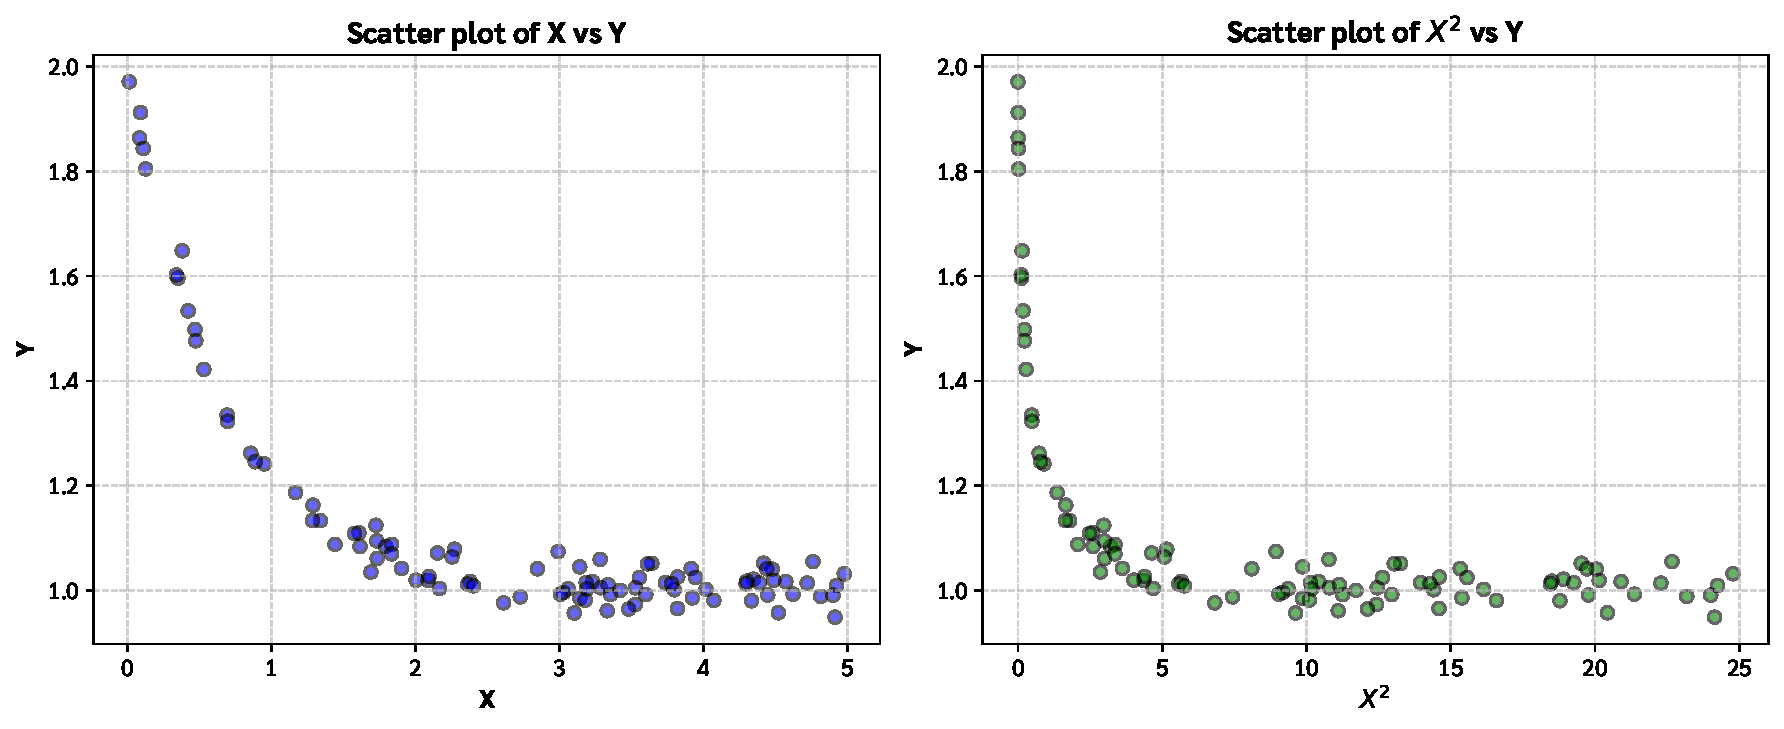
\includegraphics[width=0.85\textwidth]{plot_1_eda.pdf}
    \caption{การวิเคราะห์ข้อมูลเบื้องต้น (EDA) แสดงความสัมพันธ์ระหว่างตัวแปร $X$ และ $Y$ (ซ้าย) และตัวแปร $X^2$ และ $Y$ (ขวา)}
\end{figure}

% ══════════════════════════════════════════════════════════════════════════════
\needspace{8\baselineskip}
\section*{1. ฟังก์ชันความสูญเสีย (Loss Function)}

สำหรับโมเดล $\hat{y}_i = C_0 + C_1 e^{C_2 x_i}$ เราใช้ฟังก์ชันความสูญเสียแบบ \textbf{Mean Squared Error (MSE)} โดยใช้ตัวหารเป็น $2n$ เพื่อความสะดวกในการหาอนุพันธ์:

\[
  L(C_0, C_1, C_2) = \frac{1}{2n} \sum_{i=1}^{n} \left( y_i - \hat{y}_i \right)^2
\]

เมื่อแทนค่า $\hat{y}_i$ ลงไป จะได้:

\begin{ansbox}
\[
  L(C_0, C_1, C_2) = \frac{1}{2n} \sum_{i=1}^{n} \left( y_i - (C_0 + C_1 e^{C_2 x_i}) \right)^2
\]
\end{ansbox}

% ══════════════════════════════════════════════════════════════════════════════
\needspace{10\baselineskip}
\section*{2. การหาอนุพันธ์ย่อย (Gradient of Each Coefficient)}

เพื่อใช้ Gradient Descent เราต้องหาอนุพันธ์ย่อย (Partial derivatives) ของ $L$ เทียบกับพารามิเตอร์แต่ละตัว ($C_0, C_1, C_2$) โดยอาศัยกฎลูกโซ่ (Chain Rule)

สำหรับพารามิเตอร์ $\theta$ ใดๆ:
\begin{align*}
  \frac{\partial L}{\partial \theta} &= \frac{\partial}{\partial \theta} \left[ \frac{1}{2n} \sum_{i=1}^{n} \left( y_i - \hat{y}_i \right)^2 \right] \\
  &= \frac{1}{2n} \sum_{i=1}^{n} 2\left( y_i - \hat{y}_i \right) \cdot \frac{\partial}{\partial \theta}\left( y_i - \hat{y}_i \right) \\
  &= -\frac{1}{n} \sum_{i=1}^{n} \left( y_i - \hat{y}_i \right) \cdot \frac{\partial \hat{y}_i}{\partial \theta}
\end{align*}

\noindent\rule{\textwidth}{0.1pt}\vspace{4pt}

\textbf{1) Gradient เทียบกับ $C_0$:} \\
ขั้นแรก หา $\frac{\partial \hat{y}_i}{\partial C_0}$:
\[
  \frac{\partial \hat{y}_i}{\partial C_0} = \frac{\partial}{\partial C_0}\left( C_0 + C_1 e^{C_2 x_i} \right) = 1
\]
แทนค่ากลับลงไปในสมการกฎลูกโซ่:
\begin{ansbox}
\[
  \frac{\partial L}{\partial C_0} = -\frac{1}{n} \sum_{i=1}^{n} \left( y_i - (C_0 + C_1 e^{C_2 x_i}) \right)
\]
\end{ansbox}

\textbf{2) Gradient เทียบกับ $C_1$:} \\
ขั้นแรก หา $\frac{\partial \hat{y}_i}{\partial C_1}$:
\[
  \frac{\partial \hat{y}_i}{\partial C_1} = \frac{\partial}{\partial C_1}\left( C_0 + C_1 e^{C_2 x_i} \right) = e^{C_2 x_i}
\]
แทนค่ากลับลงไปในสมการกฎลูกโซ่:
\begin{ansbox}
\[
  \frac{\partial L}{\partial C_1} = -\frac{1}{n} \sum_{i=1}^{n} \left( y_i - (C_0 + C_1 e^{C_2 x_i}) \right) e^{C_2 x_i}
\]
\end{ansbox}

\textbf{3) Gradient เทียบกับ $C_2$:} \\
ขั้นแรก หา $\frac{\partial \hat{y}_i}{\partial C_2}$ โดยใช้กฎลูกโซ่สำหรับฟังก์ชันเอกซ์โพเนนเชียล:
\[
  \frac{\partial \hat{y}_i}{\partial C_2} = \frac{\partial}{\partial C_2}\left( C_0 + C_1 e^{C_2 x_i} \right) = C_1 \cdot \frac{\partial}{\partial C_2}\left( e^{C_2 x_i} \right) = C_1 \cdot e^{C_2 x_i} \cdot \frac{\partial}{\partial C_2}(C_2 x_i) = C_1 x_i e^{C_2 x_i}
\]
แทนค่ากลับลงไปในสมการกฎลูกโซ่:
\begin{ansbox}
\[
  \frac{\partial L}{\partial C_2} = -\frac{1}{n} \sum_{i=1}^{n} \left( y_i - (C_0 + C_1 e^{C_2 x_i}) \right) C_1 x_i e^{C_2 x_i}
\]
\end{ansbox}

% ══════════════════════════════════════════════════════════════════════════════
\needspace{10\baselineskip}
\section*{3. กฎการอัปเดตพารามิเตอร์ (Update Rules)}

ในแต่ละรอบการวนซ้ำ (Iteration) $t$ พารามิเตอร์จะถูกปรับค่าตรงข้ามกับ Gradient โดยมีอัตราการเรียนรู้ (Learning Rate) $\eta$ ควบคุมขนาดของก้าว:

\begin{ansbox}
\begin{align*}
  C_0^{(t+1)} &= C_0^{(t)} - \eta \cdot \frac{\partial L}{\partial C_0} \\
  C_1^{(t+1)} &= C_1^{(t)} - \eta \cdot \frac{\partial L}{\partial C_1} \\
  C_2^{(t+1)} &= C_2^{(t)} - \eta \cdot \frac{\partial L}{\partial C_2}
\end{align*}
\end{ansbox}

% ══════════════════════════════════════════════════════════════════════════════
\needspace{8\baselineskip}
\section*{4. การเขียนโปรแกรม (Gradient Descent Implementation)}

นำสมการ Gradient ที่ได้มาเขียนในรูปแบบโค้ด (Python/NumPy) โดยกำหนด hyperparameters เพื่อให้โมเดล Exponential สามารถฟิตได้อย่างแม่นยำและเสถียร ดังนี้:
\begin{itemize}[noitemsep, topsep=2pt]
  \item อัตราการเรียนรู้ (Learning Rate, $\eta$) = $1.0$
  \item จำนวนรอบการวนซ้ำสูงสุด (Max Iterations) = $2,000$ รอบ
  \item กำหนดค่าเริ่มต้น (Initial values) $C_0 = 0.5$, $C_1 = 0.5$ และ $C_2 = 0.1$
  \item กำหนดเกณฑ์หยุดทำงาน (Tolerance) = $10^{-6}$ เพื่อใช้ทำ Early Stopping หาก Loss ไม่เปลี่ยนแปลง
\end{itemize}

กระบวนการจะทำการอัปเดตค่าพารามิเตอร์ซ้ำๆ และบันทึกค่าพารามิเตอร์กับค่า Loss ในแต่ละรอบ เพื่อนำไปประเมินประสิทธิภาพในขั้นตอนต่อไป

% ══════════════════════════════════════════════════════════════════════════════
% ══════════════════════════════════════════════════════════════════════════════
\needspace{8\baselineskip}
\section*{5. ผลลัพธ์และการแสดงภาพ (Results \& Visualizations)}

จากผลการฝึกสอนโมเดลด้วย Batch Gradient Descent พบว่าโมเดลสามารถลู่เข้าสู่จุดต่ำสุดสัมพัทธ์ (Convergence) ได้ภายใน \textbf{270 รอบ} โดยค่าความคลาดเคลื่อน (Loss) ลดลงอย่างต่อเนื่องจนเสถียร ผลการวิเคราะห์และแสดงภาพของโมเดลมี 4 ส่วนสำคัญดังต่อไปนี้:

\begin{figure}[H]
    \centering
    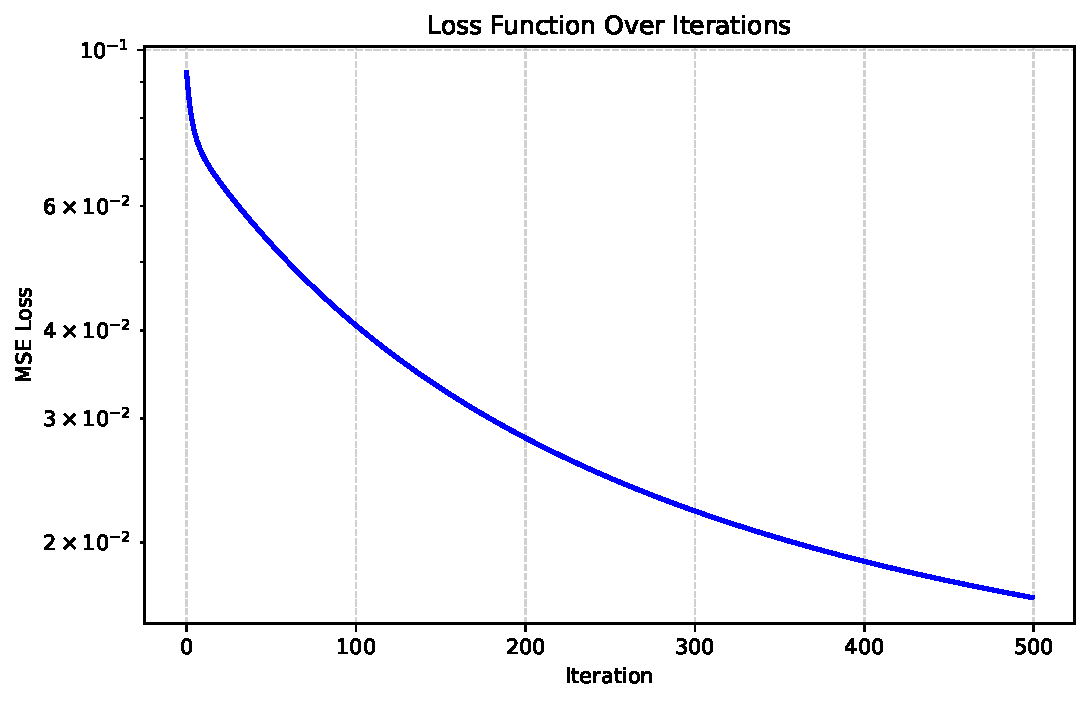
\includegraphics[width=0.78\textwidth]{plot_2_loss_curve.pdf}
    \caption{\textbf{Learning Curve (Loss vs Iterations):} แสดงการลดลงอย่างรวดเร็วของค่า MSE Loss จากเริ่มต้น $0.0465$ สู่ค่าสุดท้าย $0.0005$ (ลดลง $98.98\%$) สะท้อนว่าการเลือก Learning Rate $\eta = 1.0$ มีความเหมาะสม ทำให้โมเดลลู่เข้าได้อย่างราบเรียบโดยไม่มีอาการแกว่ง (Oscillation) หรือหลุดขอบเขต (Overshooting)}
\end{figure}

\begin{figure}[H]
    \centering
    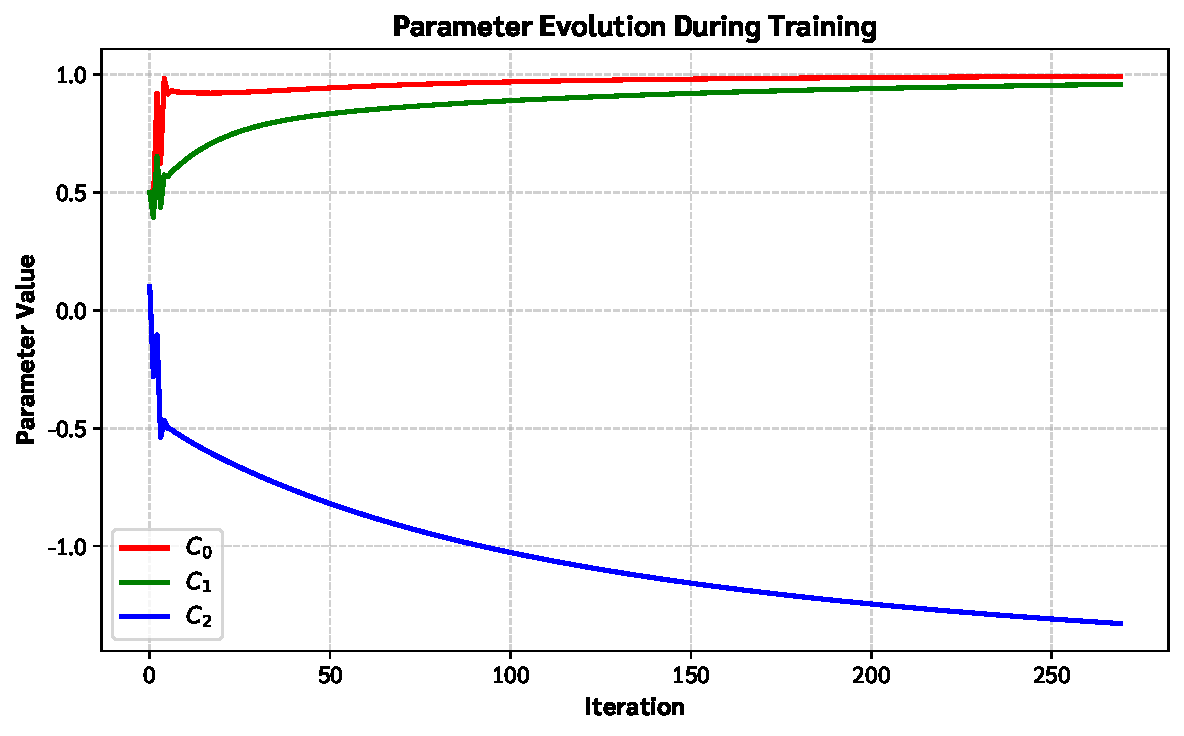
\includegraphics[width=0.78\textwidth]{plot_3_coeff_trajectory.pdf}
    \caption{\textbf{Parameter Evolution:} แสดงเส้นทางการปรับค่าสัมประสิทธิ์ทั้ง 3 ตัว ($C_0, C_1, C_2$) ในแต่ละรอบการเทรน โดย $C_0$ ปรับตัวจาก $0.5 \rightarrow 0.9927$, $C_1$ ปรับตัวจาก $0.5 \rightarrow 0.9587$ และ $C_2$ ปรับตัวจาก $0.1 \rightarrow -1.3296$ จนลู่เข้าสู่ค่าที่เสถียรอย่างมั่นคง}
\end{figure}

\begin{figure}[H]
    \centering
    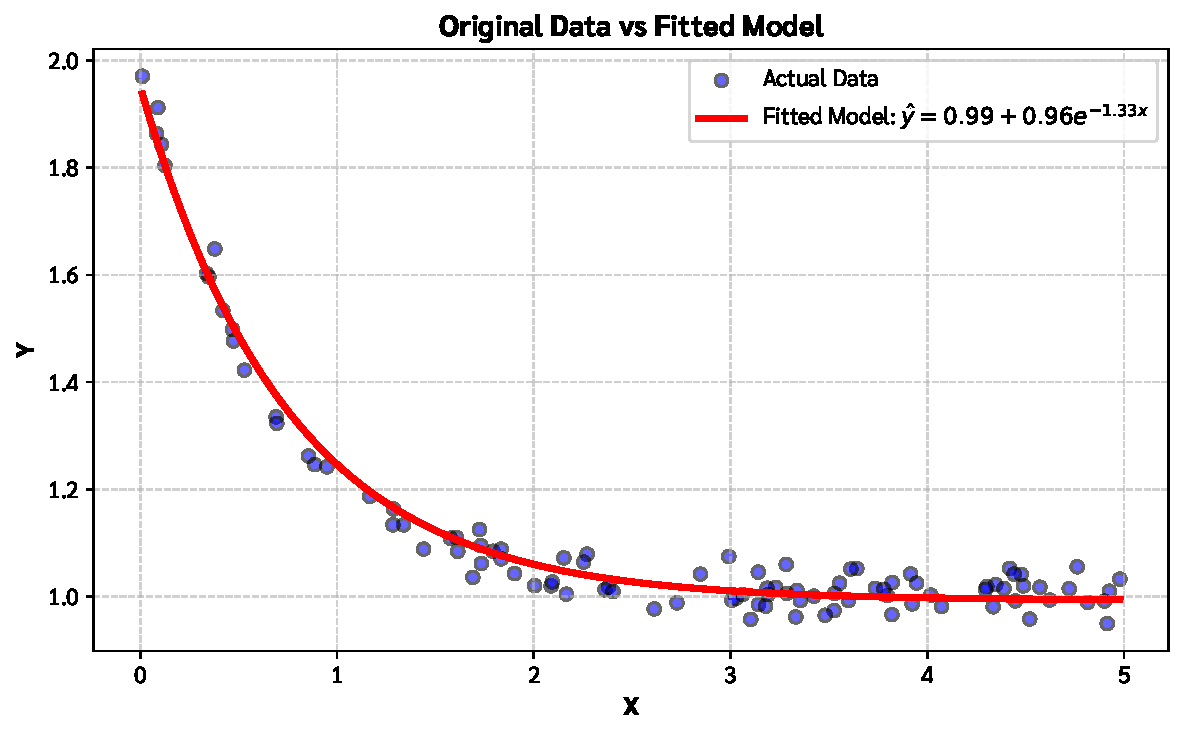
\includegraphics[width=0.78\textwidth]{plot_4_fitted_curve.pdf}
    \caption{\textbf{Original Data vs Fitted Model:} แสดงการเปรียบเทียบระหว่างข้อมูลจริง 100 จุด กับเส้นโค้งทำนายของโมเดลเอกซ์โพเนนเชียล $\hat{y} = 0.9927 + 0.9587 e^{-1.3296 x}$ ซึ่งสามารถจับแนวโน้มความสัมพันธ์แบบ Exponential Decay ของข้อมูลได้อย่างแม่นยำและกลมกลืน}
\end{figure}

\begin{figure}[H]
    \centering
    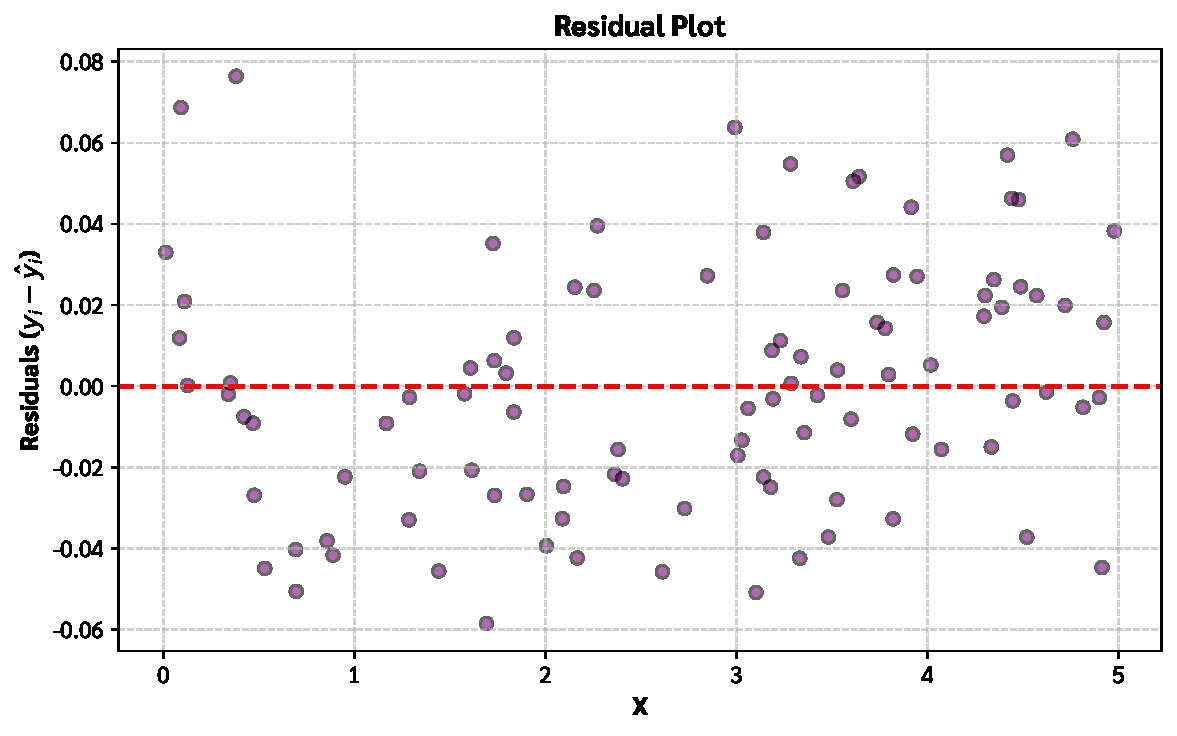
\includegraphics[width=0.78\textwidth]{plot_5_residuals.pdf}
    \caption{\textbf{Residual Plot:} แสดงการกระจายตัวของค่าเศษเหลือ ($e_i = y_i - \hat{y}_i$) พบว่าค่า Residuals กระจายตัวแบบสุ่ม (Randomly distributed) รอบแกนสมมาตร 0 และมีความแปรปรวนสม่ำเสมอ (Homoscedasticity) ไร้รูปแบบความโค้งตกค้าง ยืนยันว่าโมเดล Exponential เหมาะสมกับข้อมูลชุดนี้}
\end{figure}

% ══════════════════════════════════════════════════════════════════════════════
\needspace{8\baselineskip}
\section*{Extra: การประเมินประสิทธิภาพของโมเดล\\ \large(Mathematical Evaluation)}

เพื่อประเมินความแม่นยำของแบบจำลอง (Goodness of Fit) ในการทำนายค่า $y$ เราใช้ตัวชี้วัดคือ \textbf{Coefficient of Determination ($R^2$)} ซึ่งมีสูตรทางคณิตศาสตร์ดังนี้:
\[
  R^2 = 1 - \frac{SS_{res}}{SS_{tot}}
\]
โดยที่:
\begin{itemize}[noitemsep, topsep=2pt]
  \item \textbf{Residual Sum of Squares ($SS_{res}$):} ผลรวมกำลังสองของความคลาดเคลื่อน
  \[ SS_{res} = \sum_{i=1}^{n} \left( y_i - \hat{y}_i \right)^2 \approx 0.0948 \]
  \item \textbf{Total Sum of Squares ($SS_{tot}$):} ผลรวมกำลังสองของความแปรปรวนทั้งหมดของข้อมูล
  \[ SS_{tot} = \sum_{i=1}^{n} \left( y_i - \bar{y} \right)^2 \approx 5.2020 \]
\end{itemize}

แทนค่าในสูตร:
\[
  R^2 = 1 - \frac{0.0948}{5.2020} = 1 - 0.0182 = 0.9818
\]

\begin{ansbox}
\textbf{สรุป Extra:} \quad $\boxed{R^2 \approx 0.9818 \text{ (หรือ } 98.18\%)}$

\textbf{การตีความค่า $R^2$:} หมายความว่า \textbf{98.18\% ของความแปรปรวนในตัวแปรเป้าหมาย $Y$ สามารถอธิบายได้ด้วยตัวแปร $X$ ผ่านโมเดล Exponential ที่เทรนขึ้น} บ่งชี้ว่าแบบจำลองมีความแม่นยำและมีความสามารถในการฟิตข้อมูลอยู่ในระดับดีเยี่ยม
\end{ansbox}

% ══════════════════════════════════════════════════════════════════════════════
\needspace{8\baselineskip}
\section*{สรุปผลลัพธ์ (Summary of Results)}

\begin{table}[H]
\centering
\begin{tabular}{l l}
\toprule
\textbf{หัวข้อ} & \textbf{ผลลัพธ์และคำตอบ} \\
\midrule
\textbf{Task 1} & Loss Function: $L(C_0, C_1, C_2) = \frac{1}{2n} \sum_{i=1}^{n} \left( y_i - (C_0 + C_1 e^{C_2 x_i}) \right)^2$ \\[4pt]
\textbf{Task 2} & Partial Derivative Gradients: \\
                & \quad $\frac{\partial L}{\partial C_0} = -\frac{1}{n} \sum_{i=1}^{n} (y_i - \hat{y}_i)$ \\[2pt]
                & \quad $\frac{\partial L}{\partial C_1} = -\frac{1}{n} \sum_{i=1}^{n} (y_i - \hat{y}_i) e^{C_2 x_i}$ \\[2pt]
                & \quad $\frac{\partial L}{\partial C_2} = -\frac{1}{n} \sum_{i=1}^{n} (y_i - \hat{y}_i) C_1 x_i e^{C_2 x_i}$ \\[4pt]
\textbf{Task 3} & Update Rules: $C_j^{(t+1)} = C_j^{(t)} - \eta \frac{\partial L}{\partial C_j} \quad (j \in \{0, 1, 2\})$ \\[4pt]
\textbf{Task 4} & การเทรน Gradient Descent ($\eta = 1.0$, Tolerance $= 10^{-6}$): \\
                & \quad ลู่เข้าสำเร็จที่รอบที่ \textbf{270} (จากขีดจำกัด 2,000 รอบ) \\[4pt]
\textbf{Task 5} & ผลลัพธ์สัมประสิทธิ์และค่า Loss: \\
                & \quad สัมประสิทธิ์: $\mathbf{C_0 \approx 0.9927}, \quad \mathbf{C_1 \approx 0.9587}, \quad \mathbf{C_2 \approx -1.3296}$ \\
                & \quad สมการโมเดล: $\mathbf{\hat{y} = 0.9927 + 0.9587 e^{-1.3296 x}}$ \\
                & \quad MSE Loss: $0.046463 \rightarrow \mathbf{0.000474}$ (ลดลง \textbf{98.98\%}) \\[4pt]
\textbf{Extra}  & Goodness of Fit: $\mathbf{R^2 \approx 0.9818 \text{ (98.18\%)}}$ โมเดลมีความแม่นยำสูงมาก \\
\bottomrule
\end{tabular}
\end{table}

\clearpage

\section*{Appendix: Full Jupyter Notebook Code \& Output}

รายละเอียดต่อไปนี้คือโค้ด Python ที่ใช้แก้ปัญหาข้างต้น พร้อมผลลัพธ์และกราฟ (พิมพ์ด้วยฟอนต์ TH Sarabun New) ซึ่งได้รันจริงจาก Jupyter Notebook

% Auto-generated notebook appendix (Assignment 2)
\begin{tcolorbox}[colback=blue!5!white,colframe=blue!75!black,title=\textbf{Jupyter Notebook: Assignment\_2\_GD.ipynb}]
โค้ดและผลลัพธ์ทั้งหมดด้านล่างเป็นการรันจริงจาก Jupyter Notebook
\end{tcolorbox}

\needspace{4\baselineskip}
\vspace{0.8em}
\begin{tcolorbox}[colback=gray!5!white,colframe=gray!50!black,boxrule=0.5pt,arc=2pt,left=4pt,right=4pt,top=4pt,bottom=4pt,breakable]
\textbf{\large 2. Library \& Font Setup}\par\smallskip
Loading required scientific libraries and configuring the system's Sarabun font to support clear typography and rendering in Matplotlib.
\end{tcolorbox}
\needspace{5\baselineskip}
\vspace{0.8em}
\needspace{5\baselineskip}
\noindent\textbf{In [1]:}
\begin{lstlisting}[style=pycode]
import numpy as np
import pandas as pd
import matplotlib.pyplot as plt
import matplotlib.font_manager as fm
import os

# --- Robust Sarabun Font Setup ---
font_dir = os.path.join(os.environ.get('LOCALAPPDATA', ''), 'Microsoft', 'Windows', 'Fonts')
sarabun_r_path = os.path.join(font_dir, 'Sarabun-Regular.ttf')
sarabun_b_path = os.path.join(font_dir, 'Sarabun-Bold.ttf')

if os.path.exists(sarabun_r_path):
    fm.fontManager.addfont(sarabun_r_path)
if os.path.exists(sarabun_b_path):
    fm.fontManager.addfont(sarabun_b_path)

plt.rcParams['font.family'] = 'Sarabun'
plt.rcParams['font.size'] = 14
plt.rcParams['axes.unicode_minus'] = False # Prevent minus sign rendering issues

print("Library and font setup complete")
\end{lstlisting}
\smallskip
\needspace{5\baselineskip}
\noindent\textbf{Out[1]:}
\begin{lstlisting}[style=output]
Library and font setup complete
\end{lstlisting}
\needspace{4\baselineskip}
\vspace{0.8em}
\begin{tcolorbox}[colback=gray!5!white,colframe=gray!50!black,boxrule=0.5pt,arc=2pt,left=4pt,right=4pt,top=4pt,bottom=4pt,breakable]
\textbf{\large 3. Data Loading \& Exploratory Data Analysis (EDA)}\par\smallskip
Read the data from `CPE342\_Assignment 2\_Data.csv` and display the first few rows.
\end{tcolorbox}
\needspace{5\baselineskip}
\vspace{0.8em}
\needspace{5\baselineskip}
\noindent\textbf{In [2]:}
\begin{lstlisting}[style=pycode]
# Read data
df = pd.read_csv('CPE342_Assignment 2_Data.csv')
X = df['X'].values
Y = df['Y'].values

# Display first few rows
df.head()
\end{lstlisting}
\smallskip
\needspace{5\baselineskip}
\noindent\textbf{Out[2]:}
\begin{lstlisting}[style=output]
X         Y
0  4.072280  0.981321
1  1.724332  1.124653
2  1.901981  1.042435
3  4.914068  0.949332
4  1.165868  1.186925
\end{lstlisting}
\needspace{4\baselineskip}
\vspace{0.8em}
\begin{tcolorbox}[colback=gray!5!white,colframe=gray!50!black,boxrule=0.5pt,arc=2pt,left=4pt,right=4pt,top=4pt,bottom=4pt,breakable]
Now, let's plot scatter plots to observe the relationship and trends between $X$ and $Y$.
\end{tcolorbox}
\needspace{5\baselineskip}
\vspace{0.8em}
\needspace{5\baselineskip}
\noindent\textbf{In [3]:}
\begin{lstlisting}[style=pycode]
# Plot graphs to observe trends
plt.figure(figsize=(12, 5))

# Plot X vs Y
plt.subplot(1, 2, 1)
plt.scatter(X, Y, color='blue', alpha=0.6, edgecolor='k')
plt.title('Scatter plot of X vs Y')
plt.xlabel('X')
plt.ylabel('Y')
plt.grid(True, linestyle='--', alpha=0.6)

# Plot X^2 vs Y
plt.subplot(1, 2, 2)
plt.scatter(X**2, Y, color='green', alpha=0.6, edgecolor='k')
plt.title('Scatter plot of $X^2$ vs Y')
plt.xlabel('$X^2$')
plt.ylabel('Y')
plt.grid(True, linestyle='--', alpha=0.6)

plt.tight_layout()
plt.savefig('plot_1_eda.pdf', bbox_inches='tight')
plt.show()
\end{lstlisting}
\noindent\begin{minipage}{\linewidth}
\centering
\vspace{0.4em}
\includegraphics[width=0.88\textwidth]{nb2_out_plot_1.png}
\par\vspace{0.6em}
\begin{tcolorbox}[colback=gray!5!white,colframe=gray!50!black,boxrule=0.5pt,arc=2pt,left=6pt,right=6pt,top=5pt,bottom=5pt,unbreakable]
\textbf{Figure 1 (Exploratory Data Analysis)}: Scatter plots of $X$ vs. $Y$ and $X^2$ vs. $Y$ illustrating the non-linear decaying relationship in the dataset, confirming the necessity of fitting an exponential model rather than a simple linear model.
\end{tcolorbox}
\vspace{1.0em}
\end{minipage}
\needspace{4\baselineskip}
\vspace{0.8em}
\begin{tcolorbox}[colback=gray!5!white,colframe=gray!50!black,boxrule=0.5pt,arc=2pt,left=4pt,right=4pt,top=4pt,bottom=4pt,breakable]
\textbf{\large Task 1 — Mean Squared Error (MSE) Loss Function}\par\smallskip
Given our target exponential model:
$$ \hat{y}_i = C_0 + C_1 e^{C_2 x_i} $$
We define the \textbf{Mean Squared Error (MSE)} loss function $\mathcal{L}(C_0, C_1, C_2)$ across all $n$ data points, using a conventional factor of $\frac{1}{2n}$ to simplify algebra during differentiation:
$$ \mathcal{L}(C_0, C_1, C_2) = \frac{1}{2n} \sum_{i=1}^{n} (y_i - \hat{y}_i)^2 $$
Substituting the exponential model equation $\hat{y}_i = C_0 + C_1 e^{C_2 x_i}$ into the loss function yields:
$$ \mathcal{L}(C_0, C_1, C_2) = \frac{1}{2n} \sum_{i=1}^{n} \left( y_i - \left(C_0 + C_1 e^{C_2 x_i}\right) \right)^2 $$
\end{tcolorbox}
\needspace{4\baselineskip}
\vspace{0.8em}
\begin{tcolorbox}[colback=gray!5!white,colframe=gray!50!black,boxrule=0.5pt,arc=2pt,left=4pt,right=4pt,top=4pt,bottom=4pt,breakable]
\textbf{\large Task 2 — Derivation of Partial Derivatives (Gradients)}\par\smallskip
To minimize the loss function $\mathcal{L}$ using Gradient Descent, we calculate the partial derivatives (gradients) with respect to each model parameter ($C_0, C_1, C_2$) using the \textbf{Chain Rule}.
\textbf{1. General Chain Rule Formulation:}\par\smallskip
For any parameter $\theta \in \{C_0, C_1, C_2\}$:
$$ \frac{\partial \mathcal{L}}{\partial \theta} = \frac{\partial}{\partial \theta} \left[ \frac{1}{2n} \sum_{i=1}^{n} (y_i - \hat{y}_i)^2 \right] $$
$$ = \frac{1}{2n} \sum_{i=1}^{n} \frac{\partial}{\partial \theta} (y_i - \hat{y}_i)^2 $$
$$ = \frac{1}{2n} \sum_{i=1}^{n} 2(y_i - \hat{y}_i) \cdot \frac{\partial}{\partial \theta}(y_i - \hat{y}_i) $$
$$ = \frac{1}{n} \sum_{i=1}^{n} (y_i - \hat{y}_i) \cdot \left(-\frac{\partial \hat{y}_i}{\partial \theta}\right) $$
$$ = -\frac{1}{n} \sum_{i=1}^{n} (y_i - \hat{y}_i) \frac{\partial \hat{y}_i}{\partial \theta} $$
\end{tcolorbox}
\needspace{4\baselineskip}
\vspace{0.8em}
\begin{tcolorbox}[colback=gray!5!white,colframe=gray!50!black,boxrule=0.5pt,arc=2pt,left=4pt,right=4pt,top=4pt,bottom=4pt,breakable]
\textbf{2. Gradients with respect to $C_0$ and $C_1$:}\par\smallskip
\textbf{A) Gradient with respect to $C_0$:}
First, differentiate $\hat{y}_i = C_0 + C_1 e^{C_2 x_i}$ with respect to $C_0$:
$$ \frac{\partial \hat{y}_i}{\partial C_0} = \frac{\partial}{\partial C_0} \left( C_0 + C_1 e^{C_2 x_i} \right) = 1 + 0 = 1 $$
Substituting this back into the chain rule formula:
$$ \boxed{\frac{\partial \mathcal{L}}{\partial C_0} = -\frac{1}{n} \sum_{i=1}^{n} \left( y_i - \left(C_0 + C_1 e^{C_2 x_i}\right) \right)} $$
\noindent\rule{\textwidth}{0.2pt}\par\smallskip
\textbf{B) Gradient with respect to $C_1$:}
First, differentiate $\hat{y}_i = C_0 + C_1 e^{C_2 x_i}$ with respect to $C_1$:
$$ \frac{\partial \hat{y}_i}{\partial C_1} = \frac{\partial}{\partial C_1} \left( C_0 + C_1 e^{C_2 x_i} \right) = 0 + e^{C_2 x_i} = e^{C_2 x_i} $$
Substituting this back into the chain rule formula:
$$ \boxed{\frac{\partial \mathcal{L}}{\partial C_1} = -\frac{1}{n} \sum_{i=1}^{n} \left( y_i - \left(C_0 + C_1 e^{C_2 x_i}\right) \right) e^{C_2 x_i}} $$
\end{tcolorbox}
\needspace{4\baselineskip}
\vspace{0.8em}
\begin{tcolorbox}[colback=gray!5!white,colframe=gray!50!black,boxrule=0.5pt,arc=2pt,left=4pt,right=4pt,top=4pt,bottom=4pt,breakable]
\textbf{3. Gradient with respect to $C_2$:}\par\smallskip
First, differentiate $\hat{y}_i = C_0 + C_1 e^{C_2 x_i}$ with respect to $C_2$:
$$ \frac{\partial \hat{y}_i}{\partial C_2} = \frac{\partial}{\partial C_2} \left( C_0 + C_1 e^{C_2 x_i} \right) = 0 + C_1 \frac{\partial}{\partial C_2} \left( e^{C_2 x_i} \right) $$
Using the exponential derivative chain rule $\frac{d}{du}(e^u) = e^u \frac{du}{dx}$:
$$ \frac{\partial}{\partial C_2} \left( e^{C_2 x_i} \right) = e^{C_2 x_i} \cdot \frac{\partial}{\partial C_2}(C_2 x_i) = x_i e^{C_2 x_i} $$
$$ \Rightarrow \frac{\partial \hat{y}_i}{\partial C_2} = C_1 x_i e^{C_2 x_i} $$
Substituting this back into the chain rule formula:
$$ \boxed{\frac{\partial \mathcal{L}}{\partial C_2} = -\frac{1}{n} \sum_{i=1}^{n} \left( y_i - \left(C_0 + C_1 e^{C_2 x_i}\right) \right) C_1 x_i e^{C_2 x_i}} $$
\end{tcolorbox}
\needspace{4\baselineskip}
\vspace{0.8em}
\begin{tcolorbox}[colback=gray!5!white,colframe=gray!50!black,boxrule=0.5pt,arc=2pt,left=4pt,right=4pt,top=4pt,bottom=4pt,breakable]
\textbf{4. Summary of Complete Gradients:}\par\smallskip
$$
\begin{aligned}
\frac{\partial \mathcal{L}}{\partial C_0} &= -\frac{1}{n} \sum_{i=1}^{n} (y_i - \hat{y}_i) \\[8pt]
\frac{\partial \mathcal{L}}{\partial C_1} &= -\frac{1}{n} \sum_{i=1}^{n} (y_i - \hat{y}_i) e^{C_2 x_i} \\[8pt]
\frac{\partial \mathcal{L}}{\partial C_2} &= -\frac{1}{n} \sum_{i=1}^{n} (y_i - \hat{y}_i) C_1 x_i e^{C_2 x_i}
\end{aligned}
$$
\end{tcolorbox}
\needspace{4\baselineskip}
\vspace{0.8em}
\begin{tcolorbox}[colback=gray!5!white,colframe=gray!50!black,boxrule=0.5pt,arc=2pt,left=4pt,right=4pt,top=4pt,bottom=4pt,breakable]
\textbf{\large Task 3 — Parameter Update Rules}\par\smallskip
In each iteration $t$ of Gradient Descent, the model parameters are updated simultaneously by moving in the negative direction of their respective gradients, scaled by the learning rate $\eta$:
$$ \theta^{(t+1)} = \theta^{(t)} - \eta \nabla_{\theta} \mathcal{L} $$
Specifically, for each coefficient:
$$ C_0^{(t+1)} = C_0^{(t)} - \eta \frac{\partial \mathcal{L}}{\partial C_0} $$
$$ C_1^{(t+1)} = C_1^{(t)} - \eta \frac{\partial \mathcal{L}}{\partial C_1} $$
$$ C_2^{(t+1)} = C_2^{(t)} - \eta \frac{\partial \mathcal{L}}{\partial C_2} $$
\textbf{Where:}
\begin{itemize}
\item $C_0^{(t)}, C_1^{(t)}, C_2^{(t)}$: Current coefficient values at iteration $t$
\item $\eta$: Learning rate (step size hyperparameter)
\item $\frac{\partial \mathcal{L}}{\partial C_0}, \frac{\partial \mathcal{L}}{\partial C_1}, \frac{\partial \mathcal{L}}{\partial C_2}$: Partial derivative gradients calculated over all $n$ data points
\end{itemize}
\end{tcolorbox}
\needspace{4\baselineskip}
\vspace{0.8em}
\begin{tcolorbox}[colback=gray!5!white,colframe=gray!50!black,boxrule=0.5pt,arc=2pt,left=4pt,right=4pt,top=4pt,bottom=4pt,breakable]
\textbf{\large Task 4 — Gradient Descent Implementation}\par\smallskip
We will now implement the Gradient Descent algorithm in Python using NumPy based on our derived mathematical formulas.
\textbf{Hyperparameters \& Initial Conditions:}
\begin{itemize}
\item Learning Rate ($\eta$) = `1.0`
\item Maximum Iterations (`max\_iterations`) = `2000`
\item Convergence Tolerance (`tolerance`) = `1e-6`
\item Initial Parameter Guesses: $C_0 = 0.5, C_1 = 0.5, C_2 = 0.1$
\end{itemize}
\end{tcolorbox}
\needspace{5\baselineskip}
\vspace{0.8em}
\needspace{5\baselineskip}
\noindent\textbf{In [4]:}
\begin{lstlisting}[style=pycode]
# Initialize hyperparameters
learning_rate = 1.0
max_iterations = 2000
tolerance = 1e-6

# Initialize coefficients
C0, C1, C2 = 0.5, 0.5, 0.1
n = len(X)

# Lists to store history for visualization
history_loss = []
history_C0, history_C1, history_C2 = [], [], []

# Gradient Descent Loop
for i in range(max_iterations):
    # Calculate predictions using the exponential model
    exp_term = np.exp(C2 * X)
    Y_pred = C0 + C1 * exp_term
    
    # Calculate Error
    error = Y - Y_pred
    
    # Calculate MSE Loss (using 1/(2n))
    loss = (1 / (2 * n)) * np.sum(error**2)
    
    # Store history
    history_loss.append(loss)
    history_C0.append(C0)
    history_C1.append(C1)
    history_C2.append(C2)
    
    # Calculate Gradients
    grad_C0 = -(1 / n) * np.sum(error)
    grad_C1 = -(1 / n) * np.sum(error * exp_term)
    grad_C2 = -(1 / n) * np.sum(error * C1 * X * exp_term)
    
    # Update coefficients
    C0 -= learning_rate * grad_C0
    C1 -= learning_rate * grad_C1
    C2 -= learning_rate * grad_C2
    
    # Early stopping condition
    if i > 0 and abs(history_loss[-1] - history_loss[-2]) < tolerance:
        print(f"Converged at iteration {i}")
        break

print(f"Training completed in {len(history_loss)} iterations.")
print(f"Final Parameters: C0 = {C0:.4f}, C1 = {C1:.4f}, C2 = {C2:.4f}")
print(f"Final MSE Loss: {history_loss[-1]:.4f}")
\end{lstlisting}
\smallskip
\needspace{5\baselineskip}
\noindent\textbf{Out[4]:}
\begin{lstlisting}[style=output]
Converged at iteration 269
Training completed in 270 iterations.
Final Parameters: C0 = 0.9927, C1 = 0.9587, C2 = -1.3296
Final MSE Loss: 0.0005
\end{lstlisting}
\needspace{4\baselineskip}
\vspace{0.8em}
\begin{tcolorbox}[colback=gray!5!white,colframe=gray!50!black,boxrule=0.5pt,arc=2pt,left=4pt,right=4pt,top=4pt,bottom=4pt,breakable]
\textbf{\large Task 5 — Results \& Visualizations}\par\smallskip
In this section, we analyze the training behavior and diagnostic performance of our model through dedicated visualizations.
\end{tcolorbox}
\needspace{5\baselineskip}
\vspace{0.8em}
\needspace{5\baselineskip}
\noindent\textbf{In [5]:}
\begin{lstlisting}[style=pycode]
# Plot 1: Learning Curve
plt.figure(figsize=(8, 5))
plt.plot(range(len(history_loss)), history_loss, 'b-', linewidth=2)
plt.xlabel('Iteration')
plt.ylabel('MSE Loss')
plt.title('Loss Function Over Iterations')
plt.grid(True, linestyle='--', alpha=0.6)
plt.yscale('log')
plt.savefig('plot_2_loss_curve.pdf', bbox_inches='tight')
plt.show()
\end{lstlisting}
\noindent\begin{minipage}{\linewidth}
\centering
\vspace{0.4em}
\includegraphics[width=0.88\textwidth]{nb2_out_plot_2.png}
\par\vspace{0.6em}
\begin{tcolorbox}[colback=gray!5!white,colframe=gray!50!black,boxrule=0.5pt,arc=2pt,left=6pt,right=6pt,top=5pt,bottom=5pt,unbreakable]
\textbf{Figure 2 (Learning Curve)}: Plot of MSE Loss over iterations (logarithmic scale) demonstrating rapid, monotonic convergence of the Gradient Descent algorithm from $0.0465 \rightarrow 0.0005$ (a $98.98\%$ reduction).
\end{tcolorbox}
\vspace{1.0em}
\end{minipage}
\needspace{5\baselineskip}
\vspace{0.8em}
\needspace{5\baselineskip}
\noindent\textbf{In [6]:}
\begin{lstlisting}[style=pycode]
# Plot 2: Convergence of parameters
plt.figure(figsize=(8, 5))
plt.plot(range(len(history_C0)), history_C0, 'r-', label='$C_0$', linewidth=2)
plt.plot(range(len(history_C1)), history_C1, 'g-', label='$C_1$', linewidth=2)
plt.plot(range(len(history_C2)), history_C2, 'b-', label='$C_2$', linewidth=2)
plt.xlabel('Iteration')
plt.ylabel('Parameter Value')
plt.title('Parameter Evolution During Training')
plt.legend(fontsize=12)
plt.grid(True, linestyle='--', alpha=0.6)
plt.savefig('plot_3_coeff_trajectory.pdf', bbox_inches='tight')
plt.show()
\end{lstlisting}
\noindent\begin{minipage}{\linewidth}
\centering
\vspace{0.4em}
\includegraphics[width=0.88\textwidth]{nb2_out_plot_3.png}
\par\vspace{0.6em}
\begin{tcolorbox}[colback=gray!5!white,colframe=gray!50!black,boxrule=0.5pt,arc=2pt,left=6pt,right=6pt,top=5pt,bottom=5pt,unbreakable]
\textbf{Figure 3 (Parameter Evolution)}: Trajectories of coefficients $C_0, C_1, C_2$ across iterations, showing smooth and stable convergence from initial guesses $(0.5, 0.5, 0.1)$ toward optimal parameters $(0.9927, 0.9587, -1.3296)$.
\end{tcolorbox}
\vspace{1.0em}
\end{minipage}
\needspace{5\baselineskip}
\vspace{0.8em}
\needspace{5\baselineskip}
\noindent\textbf{In [7]:}
\begin{lstlisting}[style=pycode]
# Plot 3: Fitted Curve vs Actual Data
plt.figure(figsize=(8, 5))
x_line = np.linspace(min(X), max(X), 100)
y_line = C0 + C1 * np.exp(C2 * x_line)
plt.scatter(X, Y, color='blue', alpha=0.6, label='Actual Data', edgecolor='k')
plt.plot(x_line, y_line, 'r-', linewidth=3, label=f'Fitted Model: $\\\hat{{y}} = {C0:.2f} + {C1:.2f}e^{{{C2:.2f}x}}$')
plt.xlabel('X')
plt.ylabel('Y')
plt.title('Original Data vs Fitted Model')
plt.legend(fontsize=12)
plt.grid(True, linestyle='--', alpha=0.6)
plt.savefig('plot_4_fitted_curve.pdf', bbox_inches='tight')
plt.show()
\end{lstlisting}
\noindent\begin{minipage}{\linewidth}
\centering
\vspace{0.4em}
\includegraphics[width=0.88\textwidth]{nb2_out_plot_4.png}
\par\vspace{0.6em}
\begin{tcolorbox}[colback=gray!5!white,colframe=gray!50!black,boxrule=0.5pt,arc=2pt,left=6pt,right=6pt,top=5pt,bottom=5pt,unbreakable]
\textbf{Figure 4 (Fitted Exponential Model)}: Actual data points plotted against the fitted exponential curve $\hat{y} = 0.9927 + 0.9587 e^{-1.3296 x}$, showing an accurate fit that captures the non-linear decay of the dataset.
\end{tcolorbox}
\vspace{1.0em}
\end{minipage}
\needspace{5\baselineskip}
\vspace{0.8em}
\needspace{5\baselineskip}
\noindent\textbf{In [8]:}
\begin{lstlisting}[style=pycode]
# Plot 4: Residuals
plt.figure(figsize=(8, 5))
Y_pred_final = C0 + C1 * np.exp(C2 * X)
residuals = Y - Y_pred_final
plt.scatter(X, residuals, color='purple', alpha=0.6, edgecolor='k')
plt.axhline(0, color='red', linestyle='--', linewidth=2)
plt.xlabel('X')
plt.ylabel('Residuals ($y_i - \\\hat{y}_i$)')
plt.title('Residual Plot')
plt.grid(True, linestyle='--', alpha=0.6)
plt.savefig('plot_5_residuals.pdf', bbox_inches='tight')
plt.show()
\end{lstlisting}
\noindent\begin{minipage}{\linewidth}
\centering
\vspace{0.4em}
\includegraphics[width=0.88\textwidth]{nb2_out_plot_5.png}
\par\vspace{0.6em}
\begin{tcolorbox}[colback=gray!5!white,colframe=gray!50!black,boxrule=0.5pt,arc=2pt,left=6pt,right=6pt,top=5pt,bottom=5pt,unbreakable]
\textbf{Figure 5 (Residual Plot)}: Distribution of residuals ($y_i - \hat{y}_i$) scattered randomly around zero with constant variance, validating the assumption of homoscedasticity and confirming the absence of systematic bias.
\end{tcolorbox}
\vspace{1.0em}
\end{minipage}
\needspace{5\baselineskip}
\vspace{0.8em}
\needspace{5\baselineskip}
\noindent\textbf{In [9]:}
\begin{lstlisting}[style=pycode]
# Multi-panel combined summary dashboard
fig, ((ax1, ax2), (ax3, ax4)) = plt.subplots(2, 2, figsize=(15, 12))

# Plot 1: Learning Curve (Loss over Iterations)
ax1.plot(range(len(history_loss)), history_loss, 'b-', linewidth=2)
ax1.set_xlabel('Iteration')
ax1.set_ylabel('MSE Loss')
ax1.set_title('Loss Function Over Iterations')
ax1.grid(True, linestyle='--', alpha=0.6)
ax1.set_yscale('log')

# Plot 2: Convergence of parameters
ax2.plot(range(len(history_C0)), history_C0, 'r-', label='$C_0$', linewidth=2)
ax2.plot(range(len(history_C1)), history_C1, 'g-', label='$C_1$', linewidth=2)
ax2.plot(range(len(history_C2)), history_C2, 'b-', label='$C_2$', linewidth=2)
ax2.set_xlabel('Iteration')
ax2.set_ylabel('Parameter Value')
ax2.set_title('Parameter Evolution During Training')
ax2.legend()
ax2.grid(True, linestyle='--', alpha=0.6)

# Plot 3: Fitted Curve vs Actual Data
ax3.scatter(X, Y, color='blue', alpha=0.6, label='Actual Data', edgecolor='k')
ax3.plot(x_line, y_line, 'r-', linewidth=3, label=f'Fitted Model: $\\\hat{{y}} = {C0:.2f} + {C1:.2f}e^{{{C2:.2f}x}}$')
ax3.set_xlabel('X')
ax3.set_ylabel('Y')
ax3.set_title('Original Data vs Fitted Model')
ax3.legend(fontsize=12)
ax3.grid(True, linestyle='--', alpha=0.6)

# Plot 4: Residuals
ax4.scatter(X, residuals, color='purple', alpha=0.6, edgecolor='k')
ax4.axhline(0, color='red', linestyle='--', linewidth=2)
ax4.set_xlabel('X')
ax4.set_ylabel('Residuals ($y_i - \\\hat{y}_i$)')
ax4.set_title('Residual Plot')
ax4.grid(True, linestyle='--', alpha=0.6)

plt.tight_layout()
plt.show()
\end{lstlisting}
\noindent\begin{minipage}{\linewidth}
\centering
\vspace{0.4em}
\includegraphics[width=0.88\textwidth]{nb2_out_plot_6.png}
\par\vspace{0.6em}
\begin{tcolorbox}[colback=gray!5!white,colframe=gray!50!black,boxrule=0.5pt,arc=2pt,left=6pt,right=6pt,top=5pt,bottom=5pt,unbreakable]
\textbf{Figure 6 (Comprehensive Training Diagnostics)}: Multi-panel summary dashboard comparing the learning curve, parameter evolution, non-linear regression curve, and residual distribution in a unified view.
\end{tcolorbox}
\vspace{1.0em}
\end{minipage}
\needspace{4\baselineskip}
\vspace{0.8em}
\begin{tcolorbox}[colback=gray!5!white,colframe=gray!50!black,boxrule=0.5pt,arc=2pt,left=4pt,right=4pt,top=4pt,bottom=4pt,breakable]
\textbf{\large Extra: Model Evaluation (R-squared \& Summary Statistics)}\par\smallskip
To mathematically evaluate the goodness of fit for our machine learning model, we calculate the Coefficient of Determination, also known as $R^2$.
The formula for $R^2$ is:
$$ R^2 = 1 - \frac{SS_{res}}{SS_{tot}} $$
Where:
\begin{itemize}
\item \textbf{Residual Sum of Squares ($SS_{res}$)} is the sum of squared differences between actual and predicted values:
\end{itemize}
$$ SS_{res} = \sum_{i=1}^{n} (y_i - \hat{y}_i)^2 $$
\begin{itemize}
\item \textbf{Total Sum of Squares ($SS_{tot}$)} is the sum of squared differences between actual values and their sample mean ($\bar{y}$):
\end{itemize}
$$ SS_{tot} = \sum_{i=1}^{n} (y_i - \bar{y})^2 $$
A higher $R^2$ score ($0.9818$ or $98.18\%$) indicates that the exponential model captures almost all variation in the data.
\end{tcolorbox}
\needspace{5\baselineskip}
\vspace{0.8em}
\needspace{5\baselineskip}
\noindent\textbf{In [10]:}
\begin{lstlisting}[style=pycode]
# Print summary statistics
print("\n=== MODEL EVALUATION SUMMARY ===")
print(f"Fitted parameters: C0 = {C0:.6f}, C1 = {C1:.6f}, C2 = {C2:.6f}")
print(f"Total Iterations: {len(history_loss)}")
print(f"Initial loss: {history_loss[0]:.6f}")
print(f"Final loss: {history_loss[-1]:.6f}")
loss_reduction = (history_loss[0] - history_loss[-1]) / history_loss[0] * 100
print(f"Loss reduction: {loss_reduction:.2f}%")

# Calculate R-squared
Y_mean = np.mean(Y)
ss_res = np.sum((Y - Y_pred_final)**2)
ss_tot = np.sum((Y - Y_mean)**2)
r_squared = 1 - (ss_res / ss_tot)
print(f"Residual Sum of Squares (SS_res): {ss_res:.6f}")
print(f"Total Sum of Squares (SS_tot): {ss_tot:.6f}")
print(f"R-squared (R^2): {r_squared:.6f}")
\end{lstlisting}
\smallskip
\needspace{5\baselineskip}
\noindent\textbf{Out[10]:}
\begin{lstlisting}[style=output]
=== MODEL EVALUATION SUMMARY ===
Fitted parameters: C0 = 0.992665, C1 = 0.958671, C2 = -1.329637
Total Iterations: 270
Initial loss: 0.046463
Final loss: 0.000474
Loss reduction: 98.98%
Residual Sum of Squares (SS_res): 0.094527
Total Sum of Squares (SS_tot): 5.185142
R-squared (R^2): 0.981770
\end{lstlisting}
\needspace{4\baselineskip}
\vspace{0.8em}
\begin{tcolorbox}[colback=gray!5!white,colframe=gray!50!black,boxrule=0.5pt,arc=2pt,left=4pt,right=4pt,top=4pt,bottom=4pt,breakable]
\textbf{\large Summary of Results}\par\smallskip
\resizebox{\linewidth}{!}{
\begin{tabular}{l l l}
\toprule
\textbf{Task / Item} & \textbf{Formulation / Output} & \textbf{Description \& Meaning} \\
\midrule
\textbf{Task 1: Loss Function} & $\mathcal{L}(C_0, C_1, C_2) = \frac{1}{2n}\sum (y_i - (C_0 + C_1 e^{C_2 x_i}))^2$ & Mean Squared Error (MSE) objective function \\
\textbf{Task 2: Gradients} & $\nabla \mathcal{L} = \left[\frac{\partial\mathcal{L}}{\partial C_0}, \frac{\partial\mathcal{L}}{\partial C_1}, \frac{\partial\mathcal{L}}{\partial C_2}\right]^T$ & Analytical gradients derived via Chain Rule \\
\textbf{Task 3: Update Rules} & $C_j^{(t+1)} = C_j^{(t)} - \eta \frac{\partial\mathcal{L}}{\partial C_j}$ & Simultaneous parameter updates ($\eta = 1.0$) \\
\textbf{Task 4: Implementation} & Convergence in \textbf{270 iterations} & Trained using NumPy batch gradient descent \\
\textbf{Task 5: Final Model} & $\hat{y} = 0.9927 + 0.9587 e^{-1.3296 x}$ & $C_0 \approx 0.9927, C_1 \approx 0.9587, C_2 \approx -1.3296$ \\
\textbf{Task 5: Loss Reduction} & $0.046463 \rightarrow 0.000474$ & Total MSE loss reduction of \textbf{98.98\%} \\
\textbf{Extra: Goodness of Fit} & $R^2 \approx 0.9818 \text{ (98.18\%)}$ & Model explains \textbf{98.18\%} of target variance \\
\bottomrule
\end{tabular}
}
\end{tcolorbox}

\end{document}
